% \begin{figure}[!ht]
% 	\begin{minipage}[t]{0.48\columnwidth}
% 		\centering
% 		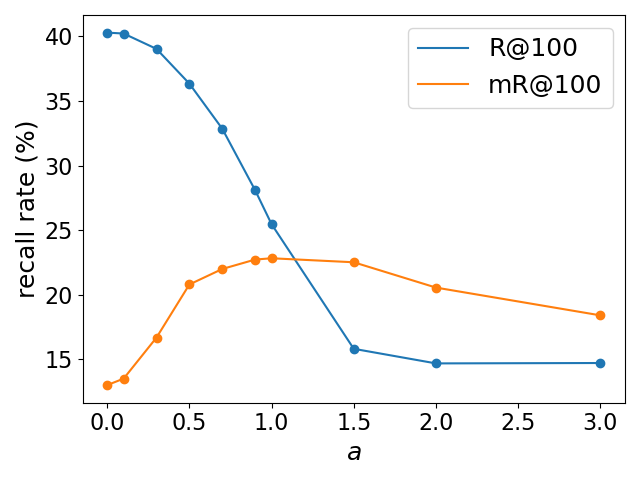
\includegraphics[width=0.9\columnwidth]{figure/train_smooth_bias}
% 		%		\caption{This fig shows the result of model trained with different smooth parameter $a$}
% 		{(a)}
% 	\end{minipage}
% 	\begin{minipage}[t]{0.48\columnwidth}
% 		\centering
% 		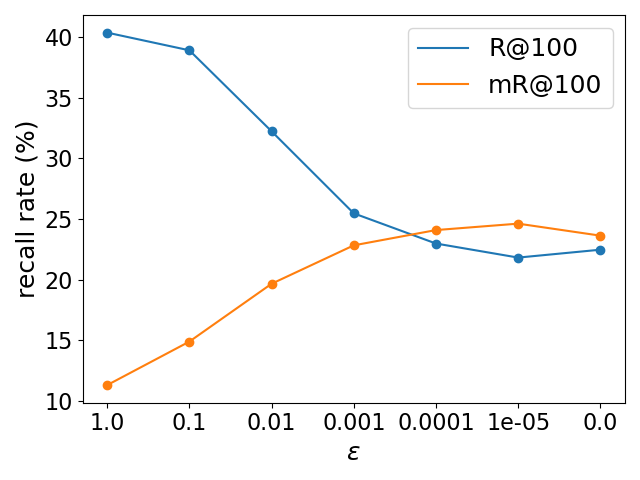
\includegraphics[width=0.9\columnwidth]{figure/train_eps}
% 		{(b)}
% 	\end{minipage}
% 	\caption{Fig (a) shows the evaluation result of the model trained with different smooth parameters $a$. Fig (b) shows the evaluation result of the model trained with different baseline parameters $\epsilon$}
% 	\label{fig:param}
% \end{figure}
\begin{figure}[!ht]
	\begin{minipage}[t]{0.49\linewidth}
		\centering
		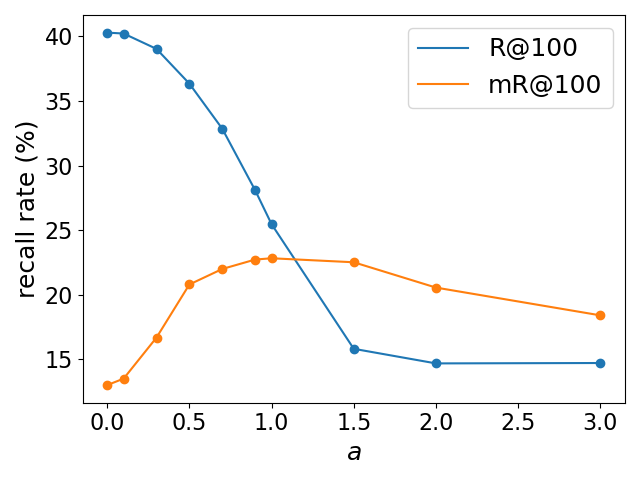
\includegraphics[width=\linewidth]{figure/train_smooth_bias}
		%		\caption{This fig shows the result of model trained with different smooth parameter $a$}
		{(a)}
	\end{minipage}
	\begin{minipage}[t]{0.49\linewidth}
		\centering
		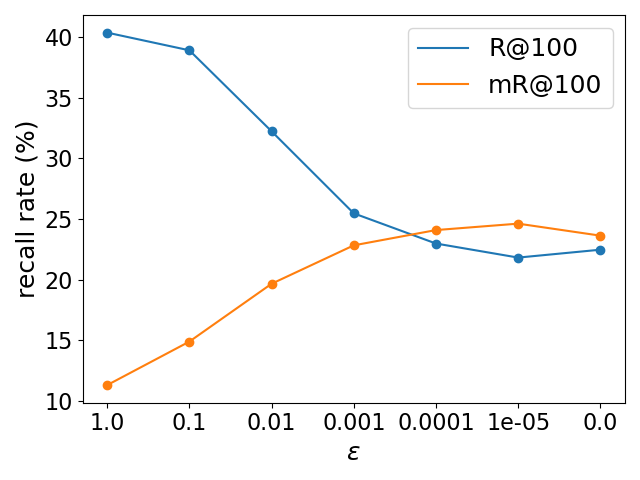
\includegraphics[width=\linewidth]{figure/train_eps}
		{(b)}
	\end{minipage}
	\caption{(a) the influence of different $a$. (b) the influence of different $\epsilon$.}
	\label{fig:param}
\end{figure}


\subsection{Ablation Studies}
In this subsection, we evaluate the influence of important hyper-parameters ($a$ and $\epsilon$) and an extended version of resistance bias, i.e., soft resistance bias. 
Besides, we compare our RTPB with several conventional imbalance learning methods on the SGG task.

\subsubsection{Hyper-parameters for Resistance Bias}

Two important hyper-parameters in RTPB, $a$ and $\epsilon$ are used to control the distribution of the resistance bias. Specifically, $a >0$ is used to adjust the divergence of the bias, while a small $\epsilon \in [0,1]$ is used to control the maximum relative difference. 
% Therefore, $\epsilon$ should be limited in $$, and it should be close to zero in order to maintain the original distribution.
%We carry out an extensive experiment to explore their role in the RTL.
We perform experiments on the SGCls task to evaluate the influence of  $a$ and $\epsilon$ in the RTPB. As shown in Figure~\ref{fig:param}(a), when increasing $a$, the overall recall rate decreases and the mean recall rate increases; when $a > 1.0$, the mean recall rate also decreases. Therefore, we use $a=1.0$ in our experiments. As shown in Figure~\ref{fig:param}(b), we find that $\epsilon = 1e-3$ achieves a good trade-off between the overall recall rate and the mean recall rate. Furthermore, we find out that when either $a = 0$ or $\epsilon \le 1$, the performance is very close to the baseline method because the resistance biases for different relationships are close to each other. 
% Based on the evaluation result, we adopt a compromise choice, where $a = 1$ and $\epsilon = 0.001$, to keep a balance between the average performance and the performance of the dominant categories.
% to show the role of $\epsilon$ in the RTL, and the result is shown in  

%\begin{figure}[t]
%	\centering
%	
\includegraphics[width=0.9\columnwidth]{train_smooth_bias}
%	\caption{This fig shows the result of model trained with different smooth parameter $a$}
%	\label{fig:tsb}
%\end{figure}
%\begin{figure}[t]
%	\centering
%	
\includegraphics[width=0.9\columnwidth]{train_eps}
%	\caption{This fig shows the result of model trained with different baseline parameter $\epsilon$}
%	\label{fig:eps}
%\end{figure}

\begin{figure}[!ht]
	\centering
	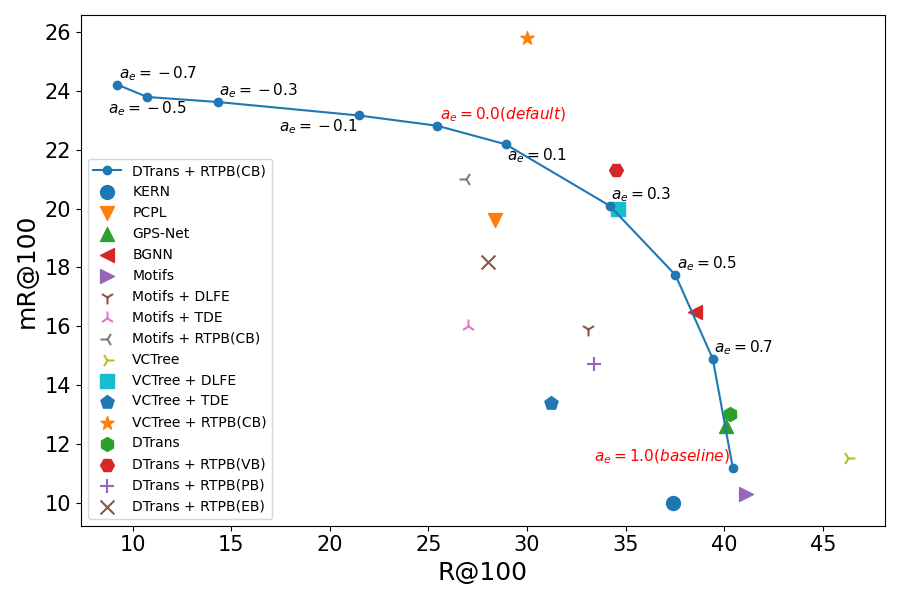
\includegraphics[width=\linewidth]{figure/R_mR_eval.png}
	\caption{The result of inference with different $a_e$.}
	\label{fig:esb}
\end{figure}

\subsubsection{Soft Resistance Bias}
% TODO: adapt for current version
To better understand how RTPB addresses the trade-off between head and tail relationships, we introduce a soft version of resistance bias during inference phase as follows.
\begin{equation}
	b_i^e = -log (\frac{w_i^{a_e}}{\sum_{j \in \mathcal{C}_r} w_j^{a_e}}+ \epsilon),
\end{equation}
where $a_e \leq a$, and $b_i^e$ is the smooth version of resistance bias. By applying a smoothed resistance bias in the inference phase, we can evaluate different impacts of RTPB on the trained model. Following the analysis of the resistance bias for adjusting the classification boundary, a smooth resistance bias reduces the margin areas of head categories from $a log\frac{w_i}{w_j}$ to $(a -a_e)log\frac{w_i}{w_j}$. Specifically, 1) when $a_e= 0$, the result is same as the original one; and 2) when $a_e = a =1$, the result is close to the baseline without RTPB, i.e., Motifs~\cite{Zellers_2018_CVPR} and DTrans.
The experimental results of different $a_e$  are shown in Figure~\ref{fig:esb}. The model used for evaluation is trained with CB and $a = 1$.
As the $a_e$ decreases, the classification margin of head categories keeps becoming larger. Therefore, the model performs worse on the few head categories but performs better on the rest tail categories. For the evaluation result, this means a consistent improvement in mean recall metric as shown in Figure~\ref{fig:esb}. Besides, the model trained with RTPB can achieve similar performance as many current SGG methods with different $a_e$. Thus RTPB can be regarded as a general baseline for  different unbiased SGG methods.
% explore how the bias  affects the model performance.
% Because we have $\epsilon = 0.001$, as the $\hat{a}$ decreases, the smoothed bias tends to be an average distribution which is equivalent to the situation of $a = 0$.

% With a small smooth weight, the classification boundary moves farther to the minority class which corresponding to a smaller resistance bias. 
% The smaller the smooth weight used in the evaluation, the larger the classification margin for those head categories.
% And this resulted in the decrease of recall metric because the performance of the head classes which dominate the dataset is getting worse. While we achieve a better result in the mean recall metric because of the better performance of all the rest classes.
\subsection{Other Cost-sensitive Methods}
% In this section, we compare our methods with several typical cost-sensitive methods for imbalance learning. We also demonstrate the performance of different variants of resistance bias.
% \section{Cost-Sensitive Methods}
As shown in Table~\ref{tab:debias}, we compare our method with the following cost-sensitive methods on the SGCls task, using our DTrans as the backbone. 
1) \textbf{Re-weighting Loss}: using the fraction of the count of each class as the weight of loss. 
% \begin{equation}
% 	\mathcal{L}_{Reweight} = \frac{1}{n}\mathcal{L}
% \end{equation}
2) \textbf{Class Balanced Re-weighting Loss} \cite{cui2019class}: using the effective number of samples to re-balance the loss. 
% The loss is calculated as
% \begin{equation}
% 	\mathcal{L}_{ClsBal} = \frac{1}{n_{eff}}\mathcal{L} = \frac{1-\beta}{1-\beta^n}\mathcal{L}
% \end{equation}
% where n is the count of the corresponding class. 
% We set the hyper-parameter $\beta= 0.999$. \\
3) \textbf{Focal Loss} \cite{Lin_2017_ICCV}: using the focal weight to adjust the losses for well-learned samples and hard samples. 
% \begin{equation}
% 	\mathcal{L}_{focal}(p_t) = -\alpha(1-p_t)^\gamma log(p_t)
% \end{equation}
% We followed the hyper-parameters (
% $\gamma = 2.0, \alpha= 0.25$) \\
4) \textbf{Label Distribution-Aware Margin Loss} \cite{cao2019learning}: using the prior margin for each class to balance the model. 
% For head classes, the margin
% The loss value for class $i$ is
% \begin{equation}
% 	\begin{split}
% 		\mathcal{L}_{LDAM}(i) = -log \frac{e^{z_i - \Delta_i}}{e^{z_i - \Delta_i} + \sum_{j\neq i}{e^{z_j}}} \\
% 		where ~ \Delta_i = \frac{C}{n_i^{1/4}}
% 	\end{split}
% \end{equation}
% where $C$ is the constant for the margin size and we set it as 0.5. This class-related loss can be regarded as a special form of our method if we set the bias corresponding to the ground truth as follow
% \begin{equation}
% 	b_i =\left\{
% 	\begin{aligned}
% 		\Delta_i, ~ & i = gt   \\
% 		0, ~        & i\neq gt
% 	\end{aligned}
% 	\right.
% \end{equation}
%(i.e. re-weighting, focal loss, and margin loss). 
%The re-weighting method.


We evaluate these methods on the SGCls task with our DTrans. As shown in Table~\ref{tab:debias}, our method outperforms the rest of the methods by a clear margin in the mean recall.
\begin{table}
\centering
	\begin{tabular}{c|ccc}
\hline
 Loss & mR@20         & mR@50         & mR@100        \\ \hline
Baseline                                            & 9.9           & 12.2          & 13.0          \\
$\mathcal{L}_{Reweight}$                            & 9.9           & 14.3          & 16.8          \\
$\mathcal{L}_{ClsBal}$                              & 12.8          & 15.5          & 17.0          \\
$\mathcal{L}_{focal}$                               & 9.1           & 11.3          & 12.1          \\
$\mathcal{L}_{LDAM}$                                & 8.4           & 10.3          & 10.8          \\
RTPB(CB)                                            & \textbf{19.1} & \textbf{21.8} & \textbf{22.8} \\ \hline
\end{tabular}
	\caption{Comparison with other cost-sensitive methods.}
	\label{tab:debias}
\end{table}



% %Besides, we 
% %\subsection{Evaluation With Smooth}

% % compare to reweight method
% compare to 